\documentclass[12pt]{article}

\usepackage{report}

\usepackage[utf8]{inputenc} % allow utf-8 input
\usepackage[T1]{fontenc}    % use 8-bit T1 fonts
\usepackage[colorlinks=true, linkcolor=black, citecolor=blue, urlcolor=blue]{hyperref}       % hyperlinks
\usepackage{url}            % simple URL typesetting
\usepackage{booktabs}       % professional-quality tables
\usepackage{amsfonts}       % blackboard math symbols
\usepackage{nicefrac}       % compact symbols for 1/2, etc.
\usepackage{microtype}      % microtypography
\usepackage{lipsum}		% Can be removed after putting your text content
\usepackage{graphicx}
\usepackage{natbib}
\usepackage{doi}
\usepackage{listings}
\usepackage{xcolor}
\usepackage{float}
\setcitestyle{aysep={,}}



\title{Project Step 2}

\author{Brian Lee, Chloe Gentry, Vinny Rose\\
\AND\\
\AND
\AND
\AND
\AND
	CS.3339 Computer Architecture\\
\AND
	Texas State University\\
}

% Uncomment to remove the date
\date{October 28, 2024}

% Uncomment to override  the `A preprint' in the header
\renewcommand{\headeright}{Project Step 2 - Group Name}
\renewcommand{\undertitle}{Smarty Pants}
\renewcommand{\shorttitle}{}

\definecolor{codegreen}{rgb}{0,0.6,0}
\definecolor{codegray}{rgb}{0.5,0.5,0.5}
\definecolor{codepurple}{rgb}{0.58,0,0.82}
\definecolor{backcolour}{rgb}{0.95,0.95,0.92}

\lstdefinestyle{mystyle}{
    backgroundcolor=\color{backcolour},   
    commentstyle=\color{codegreen},
    keywordstyle=\color{magenta},
    numberstyle=\tiny\color{codegray},
    stringstyle=\color{codepurple},
    basicstyle=\ttfamily\footnotesize,
    breakatwhitespace=false,         
    breaklines=true,                 
    captionpos=b,                    
    keepspaces=true,                 
    numbers=left,                    
    numbersep=5pt,                  
    showspaces=false,                
    showstringspaces=false,
    showtabs=false,                  
    tabsize=2
}

\lstset{style=mystyle}


\begin{document}
\maketitle

\newpage
\tableofcontents
\thispagestyle{empty}


\newpage
\setcounter{page}{1}
\section{Introduction}
In this project, we implemented essential components of a 4-bit Arithmetic Logic Unit (ALU). First, we coded 4-bit binary logic functions, including AND, NAND, OR, NOR, XOR, XNOR, and NOT, as well as a 2x4-bit input/output shifter. We then implemented 4-bit arithmetic operations such as addition, subtraction, multiplication, and division, integrating carry-in and carry-out circuits for extended accuracy. We included an extra 4-bit output for multiplication and division remainders.

Next, we tested each circuit's functionality to ensure expected behavior, followed by generating simulation waveforms to visually confirm the ALU’s performance. Finally, we compiled our work and observations into a comprehensive report, which summarizes the methods, results, and key insights gained from the project.

\section{2x4 Shift Circuit}
\label{sec:headings}

The 2x4 shift circuit takes a 4-bit input and shifts the bits left or right by up to two positions, depending on the control signal. Each shift moves the bits in the input to adjacent positions, and the vacant bits are filled with zeros. Shifting by one or two positions allows for additional flexibility in data manipulation, making the circuit versatile in operations where both single and double shifts are required.
\subsection{Shift Circuit Verilog Code}
%\lstinputlisting[language=Verilog]{2x4Shifter/shift_tb.v}

To test the Shift circuit we have created 2 registers, one for the input and one for the shifting then one wire for the output. If this circuit works properly the output should display the input shifted to the left and zeros filling the shifted positions.
%\lstinputlisting[language=Verilog]{2x4Shifter/shift_tb.v}


\subsection{Shift Circuit Waveforms}

At 0 ns, we can see that A is 0, so the output Y is 0.
\begin{figure}[H]
    \centering
%    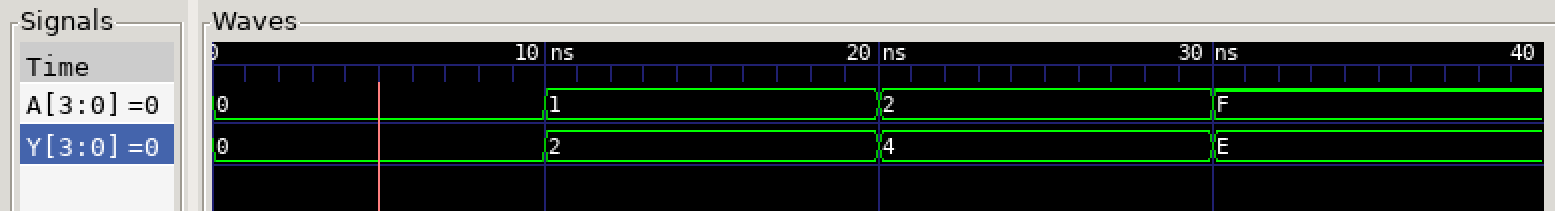
\includegraphics[width = 1.0\textwidth]{1x4bit-shift/shift_wave1.PNG}
    \caption{Shift Circuit with marker at 0ns}
    \label{fig:shift-wave1}
\end{figure}

At 10 ns, A is 1 (0001), so Y becomes 2 (0010).
\begin{figure}[H]
    \centering
%    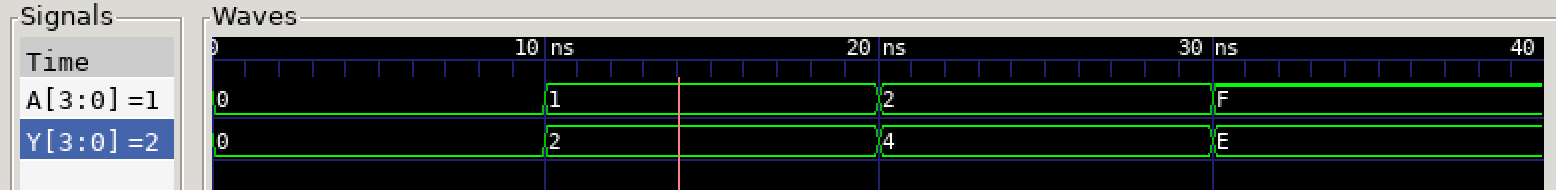
\includegraphics[width = 1.0\textwidth]{1x4bit-shift/shift_wave2.PNG}
    \caption{Shift Circuit with marker at 10ns}
    \label{fig:shift-wave2}
\end{figure}

At 20 ns, A is 2 (0010), so Y becomes 4 (0100).
\begin{figure}[H]
    \centering
%    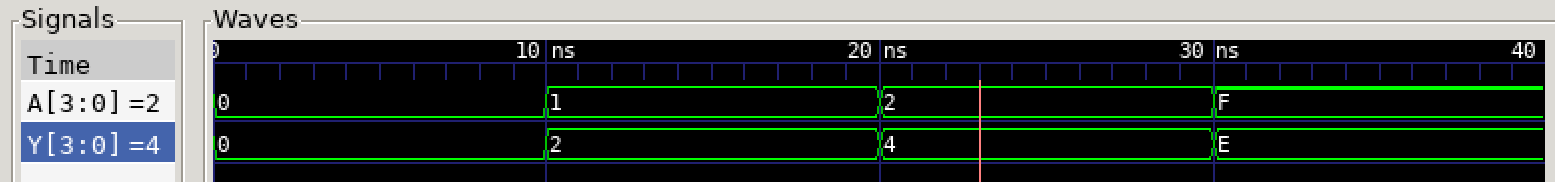
\includegraphics[width = 1.0\textwidth]{1x4bit-shift/shift_wave3.PNG}
    \caption{Shift Circuit with marker at 20ns}
    \label{fig:shift-wave3}
\end{figure}


At 30 ns, A is F (1111) so Y becomes E (1110).
\begin{figure}[H]
    \centering
%    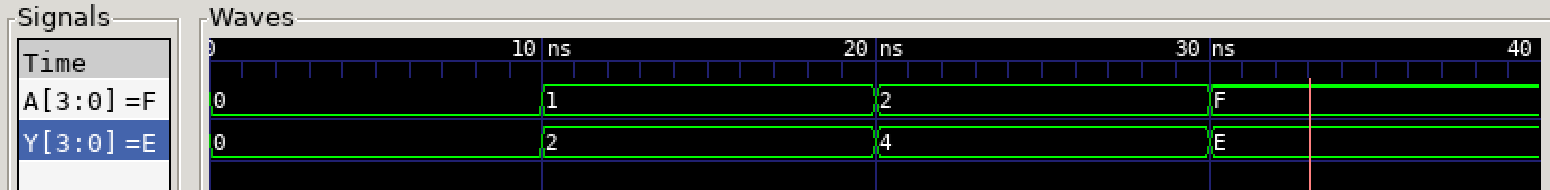
\includegraphics[width = 1.0\textwidth]{1x4bit-shift/shift_wave4.PNG}
    \caption{Shift Circuit with marker at 30ns}
    \label{fig:shift-wave4}
\end{figure}

\section{Not Circuit}
The Not circuit takes one input A, with an output Y. This will output a 0 if A is a 1, and will output 1 if A is a 0.

```\begin{figure}[H]
    \centering
%    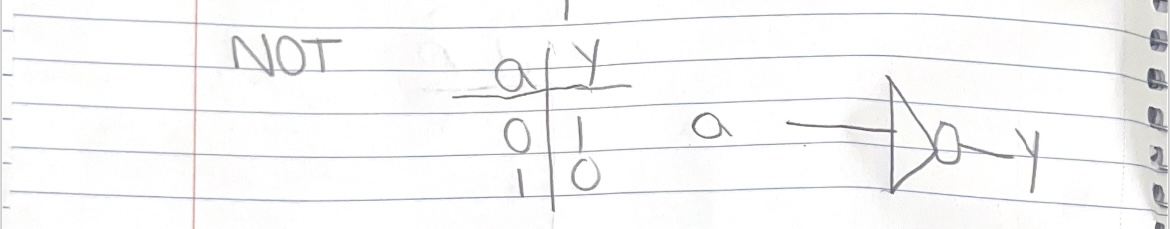
\includegraphics[width = 1.0\textwidth]{Truth-Tables/NotTT.PNG}
    \caption{Not truth table and gate}
    \label{fig:shift-table}
\end{figure}

\subsection{Not Circuit Verilog Code}
\lstinputlisting[language=Verilog]{Not/not_gate.v}

To test the Not circuit, we have created one register A, as well as a wire Y. This way we are able to take each input for A and test output for A=0 and A=1. We'll know if this is working correctly if Y returns 1 for the test where A is 0 and Y returns 0 when A is 1.
\lstinputlisting[language=Verilog]{Not/not_tb.v}

\subsection{Not Circuit Waveform}
At 0 ns, we can see that A is the 0h(0000), so the output Y is Fh(1111).
\begin{figure}[H]
    \centering
    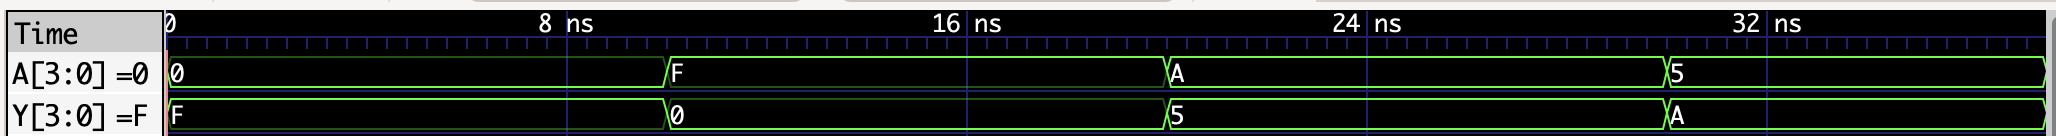
\includegraphics[width = 1.0\textwidth]{Not/Not-0ns.png}
    \caption{Not Circuit with marker at 0ns}
    \label{fig:enter-label}
\end{figure}

At 20 ns, A becomes the Ah(1010), so Y becomes the 5h(0101).
\begin{figure}[H]
    \centering
    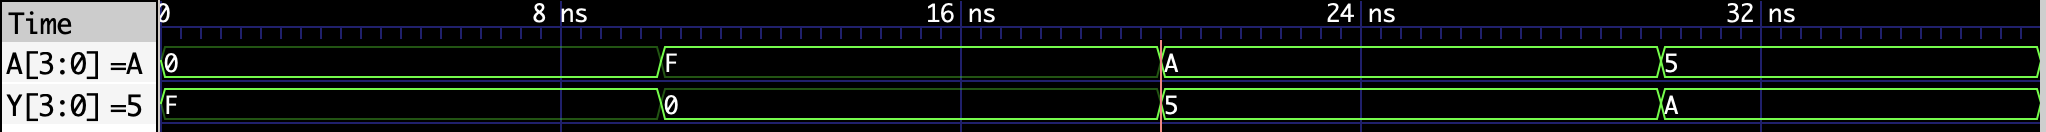
\includegraphics[width = 1.0\textwidth]{Not/Not-20ns.png}
    \caption{Not Circuit with marker at 20ns}
    \label{fig:enter-label}
\end{figure}

At 40 ns, A becomes the 5h(0101), so Y becomes the hex value Ah(1010).
\begin{figure}[H]
    \centering
    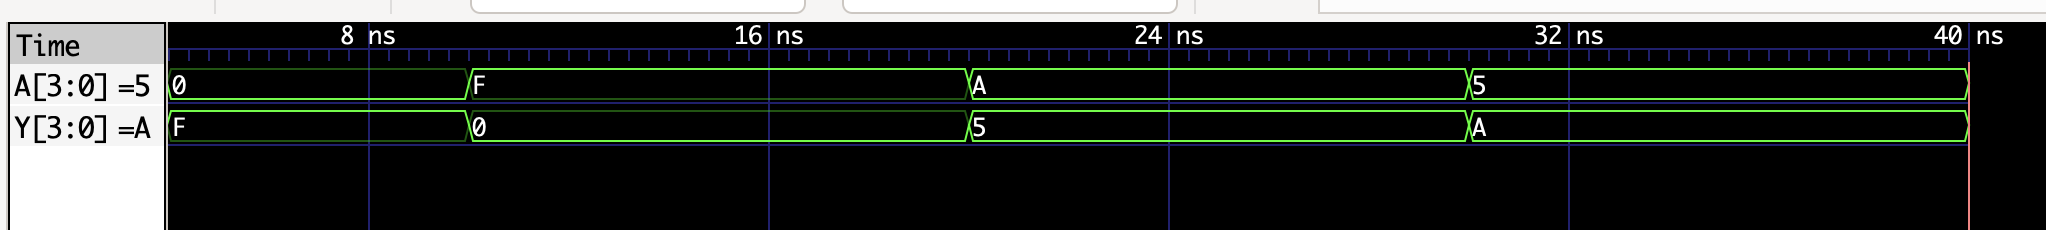
\includegraphics[width = 1.0\textwidth]{Not/Not-40ns.png}
    \caption{Not Circuit with marker at 40ns}
    \label{fig:enter-label}
\end{figure}

\section{And Circuit}

The And circuit takes two 4-bit inputs A and B, with a 4-bit output Y. A and B will undergo the bitwise And operation, and the result will be output to Y.
```\begin{figure}[H]
    \centering
    %\includegraphics[width = 1.0\textwidth]{Truth-Tables/AndTT.PNG}
    \caption{And truth table and gate}
    \label{fig:shift-table}
\end{figure}
\subsection{And Circuit Verilog Code} 
\lstinputlisting[language=Verilog]{And/and_gate.v} 

To test the And circuit, we have created two registers A and B, as well as a wire Y. We then create a for loop to produce all 16 possible values for A and B. We will know that our And circuit is behaving as expected if Y produces correct values for all combinations of A and B. For example, if A=0001 and B=0001, the expected result for Y is 0001. 
 \lstinputlisting[language=Verilog]{And/and_tb.v}

\subsection{And Circuit Waveform} 

At 1ns, A and B are both 0000, so Y is also 0000
\begin{figure}[H]
 \centering
 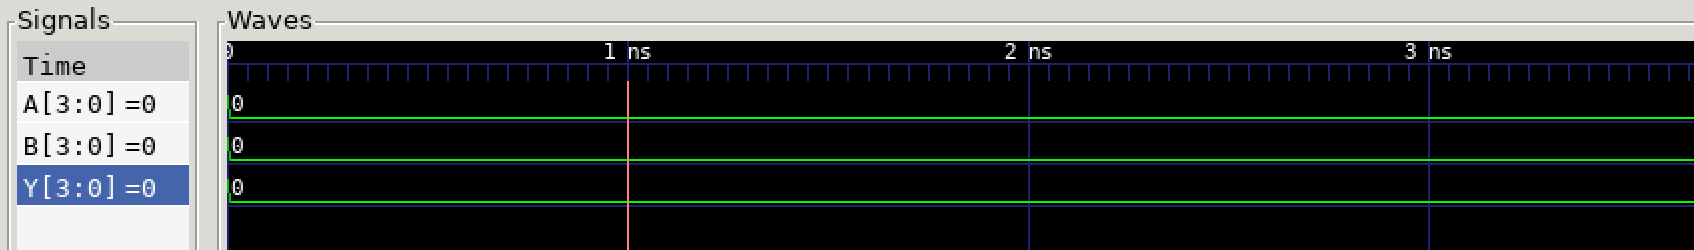
\includegraphics[width = 1.0\textwidth]{And/and_wave.png}
 \caption{And Circuit with marker at 1ns}
 \label{fig:enter-label} 
\end{figure} 

At 500ns, A=0011 and B=0010, so Y=0010
 \begin{figure}[H]
 \centering 
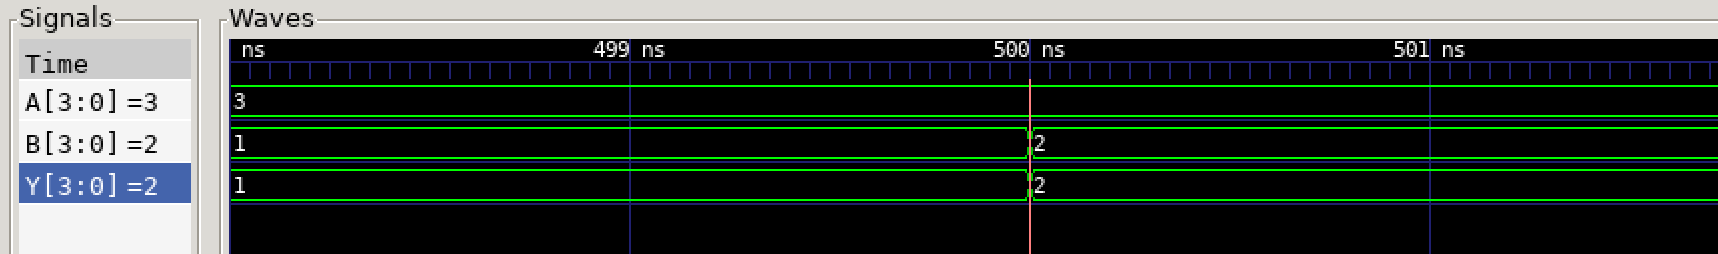
\includegraphics[width = 1.0\textwidth]{And/and_wave1.png}
 \caption{And Circuit with marker at 500ns}
 \label{fig:enter-label}
 \end{figure}

At 2550ns, A and B are both F (1111), so Y is also F (1111).
 \begin{figure}[H]
 \centering 
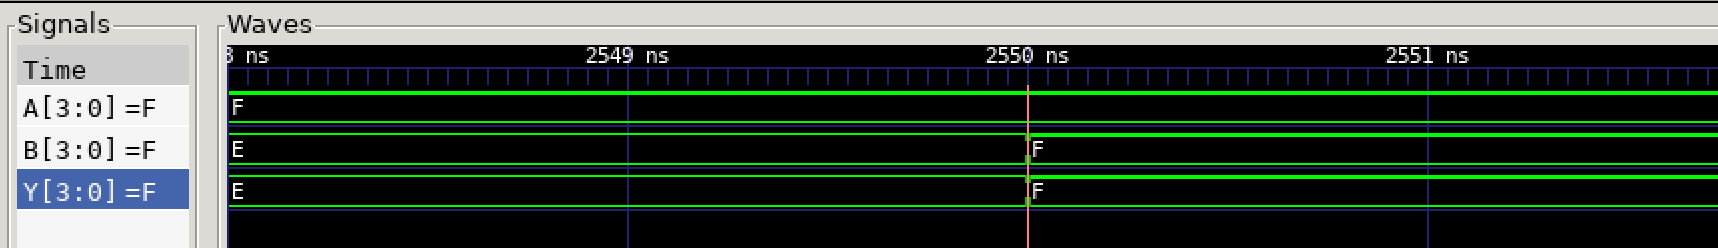
\includegraphics[width = 1.0\textwidth]{And/and_wave2.png}
 \caption{And Circuit with marker at 2550ns}
 \label{fig:enter-label}
 \end{figure}

\section{Nand Circuit}

The Nand circuit takes two 4-bit inputs A and B, with a 4-bit output Y. A and B will undergo the bitwise Nand operation, and the result will be output to Y.
\subsection{Nanad Circuit Verilog Code} 
\lstinputlisting[language=Verilog]{Nand/nand_gate.v} 

To test the Nand circuit, we have created two registers A and B, as well as a wire Y. We then create a for loop to produce all 16 possible values for A and B. We will know that our Nand circuit is behaving as expected if Y produces correct values for all combinations of A and B. For example, if A=0001 and B=0001, the expected result for Y is 1110. 
 \lstinputlisting[language=Verilog]{Nand/nand_tb.v}

\subsection{Nand Circuit Waveform} 

At 1ns, A and B are both 0000, so Y is F (1111).
\begin{figure}[H]
 \centering
 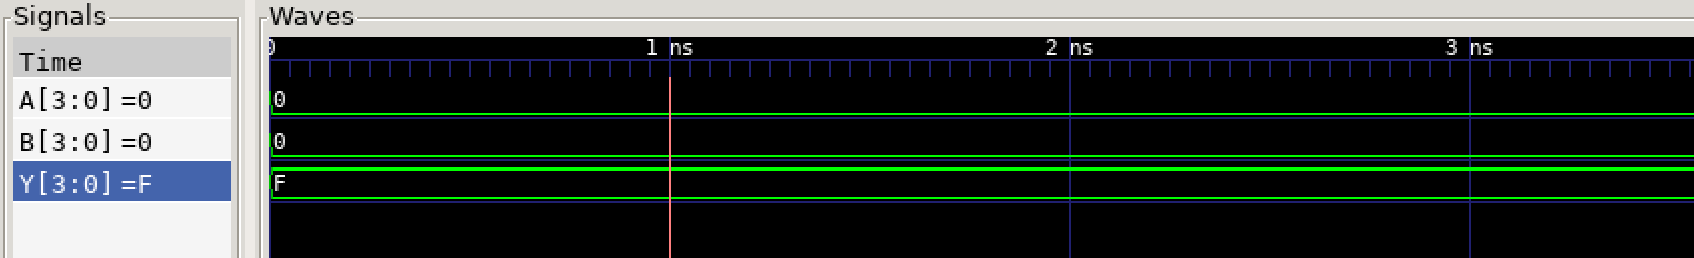
\includegraphics[width = 1.0\textwidth]{Nand/nand_wave.png}
 \caption{Nand Circuit with marker at 1ns}
 \label{fig:enter-label} 
\end{figure} 

At 500ns, A=0011 and B=0010, so Y=D (1101) 
 \begin{figure}[H]
 \centering 
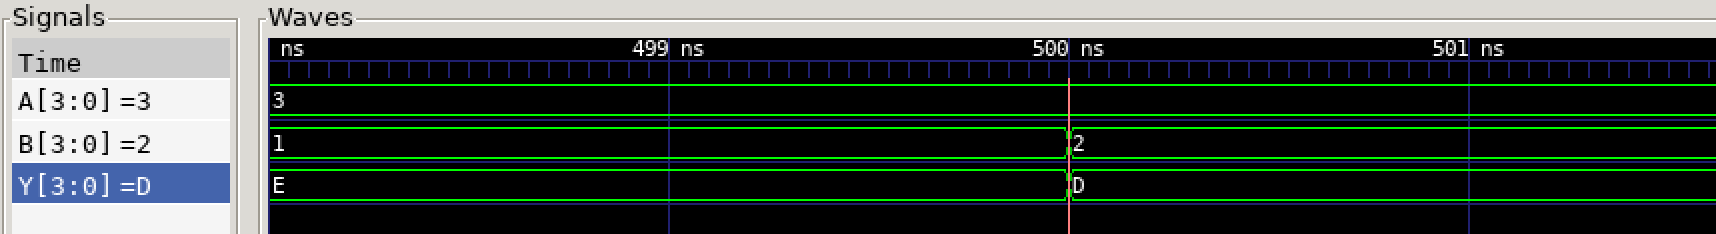
\includegraphics[width = 1.0\textwidth]{Nand/nand_wave1.png}
 \caption{Nand Circuit with marker at 500ns}
 \label{fig:enter-label}
 \end{figure}

At 2500ns, A and B are both F (1111), so Y is 0000. 
 \begin{figure}[H]
 \centering 
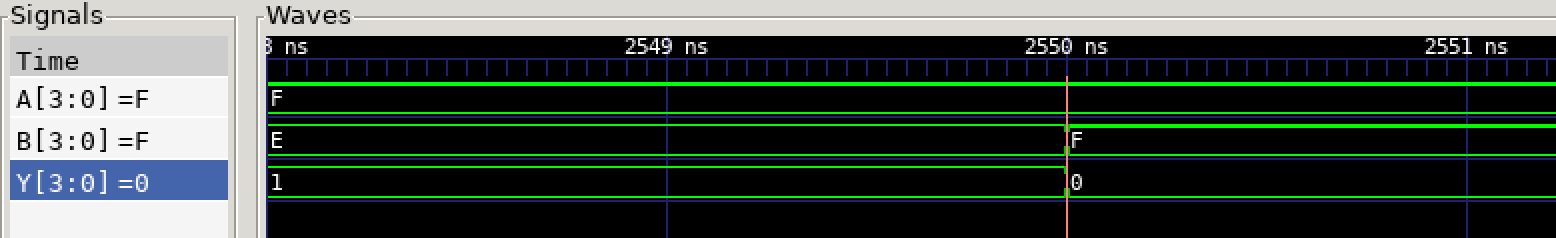
\includegraphics[width = 1.0\textwidth]{Nand/nand_wave2.png}
 \caption{Nand Circuit with marker at 560ns}
 \label{fig:enter-label}
 \end{figure}

 \section{Or Circuit}
 The Or circuit takes two 4-bit inputs A and B, and has a 4-bit output Y. Each bit of Y is the result of a bitwise OR operation applied between corresponding bits in A and B.
```\begin{figure}[H]
    \centering
    %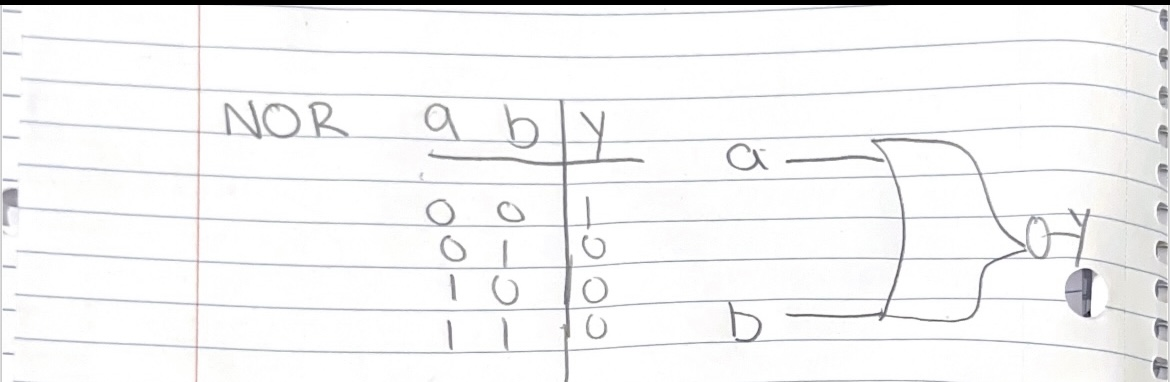
\includegraphics[width = 1.0\textwidth]{Truth-Tables/NorTT.PNG}
    \caption{Or truth table and gate}
    \label{fig:shift-table}
\end{figure}

\subsection{Or Circuit Verilog Code}
\lstinputlisting[language=Verilog]{or/or_gate.v}

To test the Nor circuit, we have created two registers, A and B, as well as a wire Y. This way we are able to take two inputs at a time and test each possible input for the circuit. We'll know if this is working correctly if Y returns 1 for the test where A and B are 0 and Y should return 0 for the rest.
%\lstinputlisting[language=Verilog]{or/or_tb.v}
\subsection{Or Circuit Waveform}

At 0 ns, A and B are 0, so Y is 1.
\begin{figure}[H]
    \centering
%    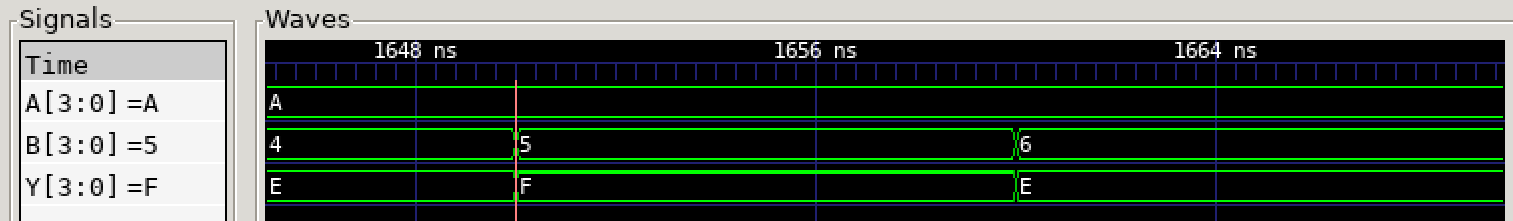
\includegraphics[width = 1.0\textwidth]{or/or_wave1.PNG}
    \caption{Nor Circuit with marker at 0ns}
    \label{fig:enter-label}
\end{figure}

At 10 ns, A is 0 and B is 1, so Y is now 0.
\begin{figure}[H]
    \centering
 %   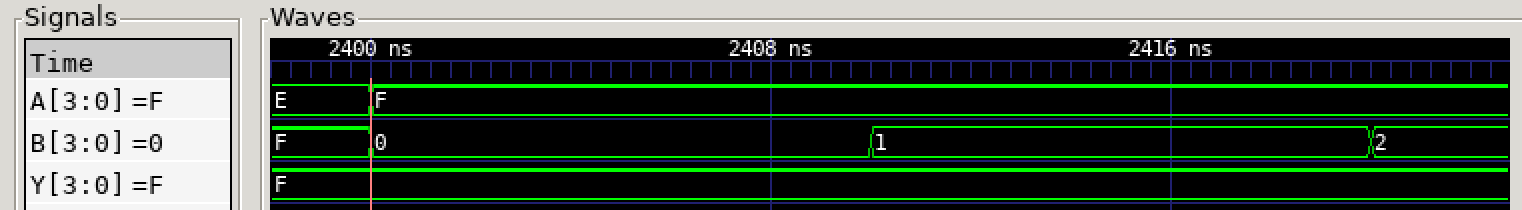
\includegraphics[width = 1.0\textwidth]{or/or_wave2.PNG}
    \caption{Nor Circuit with marker at 10ns}
    \label{fig:enter-label}
\end{figure}

At 20 ns, A is 1 and B is 0, so Y is still 0.
\begin{figure}[H]
    \centering
%    \includegraphics[width = 1.0\textwidth]{or/or_wave3.PNG}
    \caption{Nor Circuit with marker at 20ns}
    \label{fig:enter-label}
\end{figure}

At 30 ns, both A and B are 1, so Y again stays 0.
\begin{figure}[H]
    \centering
%    \includegraphics[width = 1.0\textwidth]{or/or_wave4.PNG}
    \caption{Or Circuit with marker at 30ns}
    \label{fig:enter-label}
\end{figure}

 \section{Nor Circuit}
The Nor circuit takes two inputs, A and B, with an output Y. This will output a 0 if either A or B is a 1, and will only output 1 if A and B are both 0.

```\begin{figure}[H]
    \centering
    %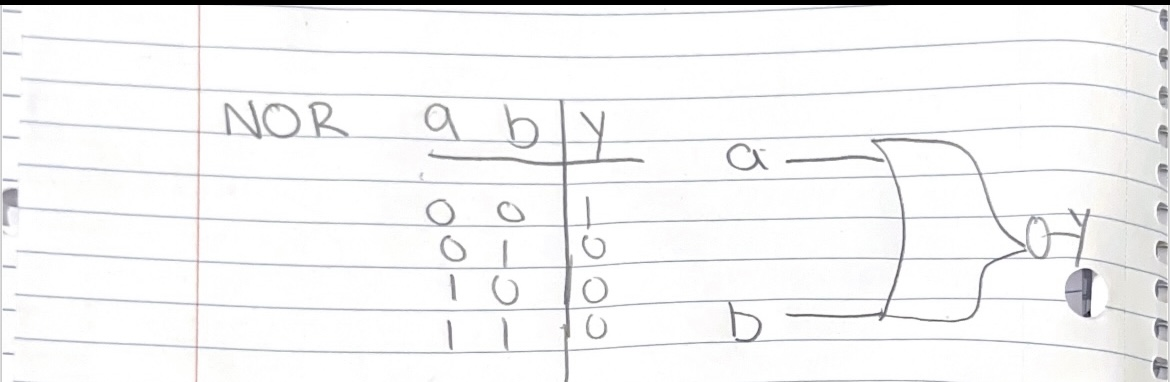
\includegraphics[width = 1.0\textwidth]{Truth-Tables/NorTT.PNG}
    \caption{Nor truth table and gate}
    \label{fig:shift-table}
\end{figure}

\subsection{Nor Circuit Verilog Code}
\lstinputlisting[language=Verilog]{nor/nor_gate.v}

To test the Nor circuit, we have created two registers, A and B, as well as a wire Y. This way we are able to take two inputs at a time and test each possible input for the circuit. We'll know if this is working correctly if Y returns 1 for the test where A and B are 0 and Y should return 0 for the rest.
%\lstinputlisting[language=Verilog]{nor/nor_tb.v}
\subsection{Nor Circuit Waveform}

At 0 ns, A and B are 0, so Y is 1.
\begin{figure}[H]
    \centering
%    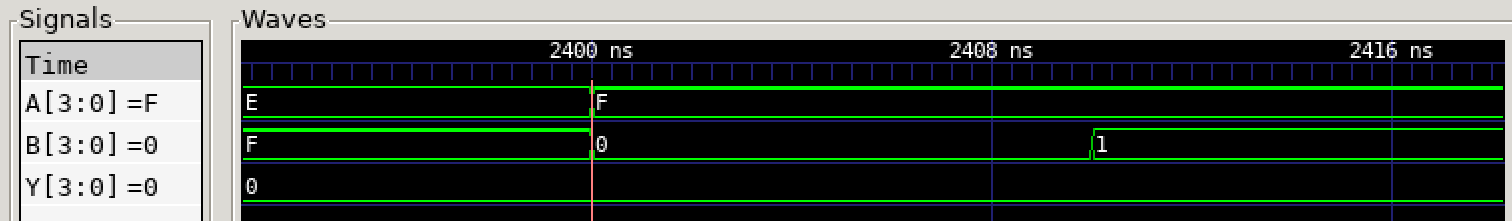
\includegraphics[width = 1.0\textwidth]{nor/nor_wave1.PNG}
    \caption{Nor Circuit with marker at 0ns}
    \label{fig:enter-label}
\end{figure}

At 10 ns, A is 0 and B is 1, so Y is now 0.
\begin{figure}[H]
    \centering
 %   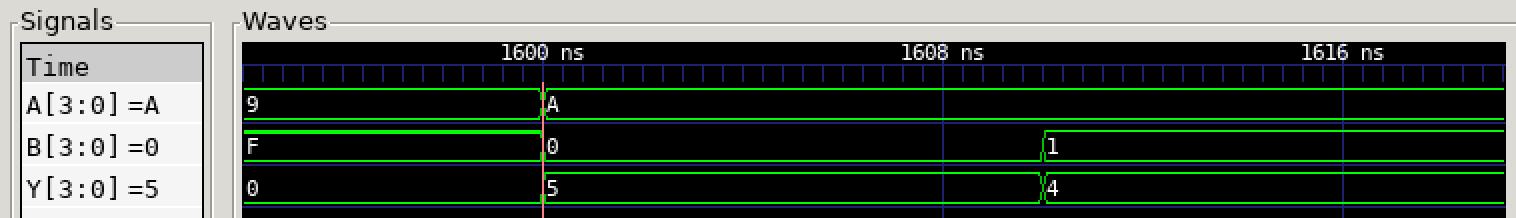
\includegraphics[width = 1.0\textwidth]{nor/nor_wave2.PNG}
    \caption{Nor Circuit with marker at 10ns}
    \label{fig:enter-label}
\end{figure}

At 20 ns, A is 1 and B is 0, so Y is still 0.
\begin{figure}[H]
    \centering
%    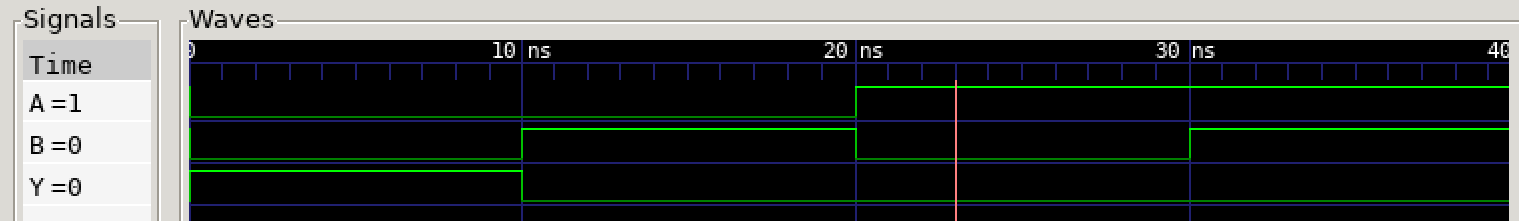
\includegraphics[width = 1.0\textwidth]{nor/nor_wave3.PNG}
    \caption{Nor Circuit with marker at 20ns}
    \label{fig:enter-label}
\end{figure}

At 30 ns, both A and B are 1, so Y again stays 0.
\begin{figure}[H]
    \centering
%    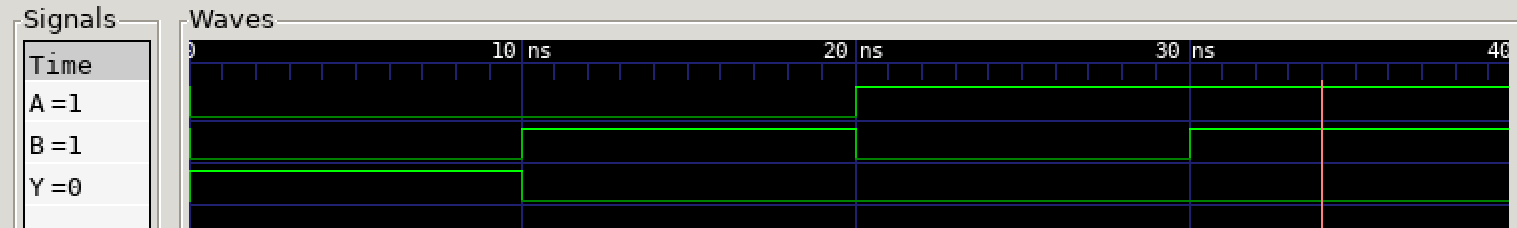
\includegraphics[width = 1.0\textwidth]{nor/nor_wave4.PNG}
    \caption{Nor Circuit with marker at 30ns}
    \label{fig:enter-label}
\end{figure}

\section{Xor Circuit}
The Xor circuit takes two 4-bit inputs A and B, with a 4-bit output Y. A and B will undergo the bitwise Xor operation, and the result will be output to Y.
\lstinputlisting[language=Verilog]{Xor/xor_gate.v} 

To test the Xor circuit, we have created two registers A and B, as well as a wire Y. We then create a for loop to produce all 16 possible values for A and B. We will know that our Xor circuit is behaving as expected if Y produces correct values for all combinations of A and B. For example, if A=1010 and B=1101, the expected result for Y is 0111. 
 \lstinputlisting[language=Verilog]{Xor/xor_tb.v}

\subsection{Xor Circuit Waveform} 

At 1ns, A and B are both 0000, so Y is also 0000.
\begin{figure}[H]
 \centering
 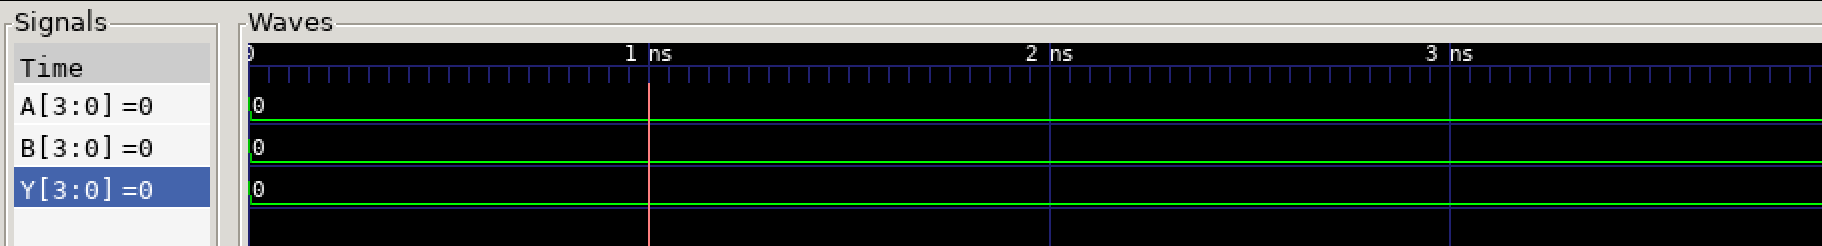
\includegraphics[width = 1.0\textwidth]{Xor/xor_wave.png}
 \caption{Xor Circuit with marker at 1ns}
 \label{fig:enter-label} 
\end{figure} 

At 500ns, A=0011 and B=0010, so Y=0001.
 \begin{figure}[H]
 \centering 
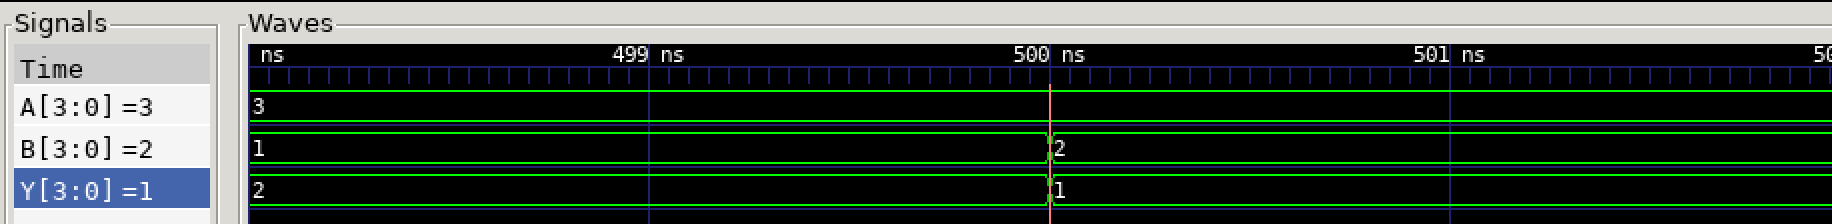
\includegraphics[width = 1.0\textwidth]{Xor/xor_wave1.png}
 \caption{Xor Circuit with marker at 500ns}
 \label{fig:enter-label}
 \end{figure}

At 2500ns, A and B are both F, so Y=0000.
 \begin{figure}[H]
 \centering 
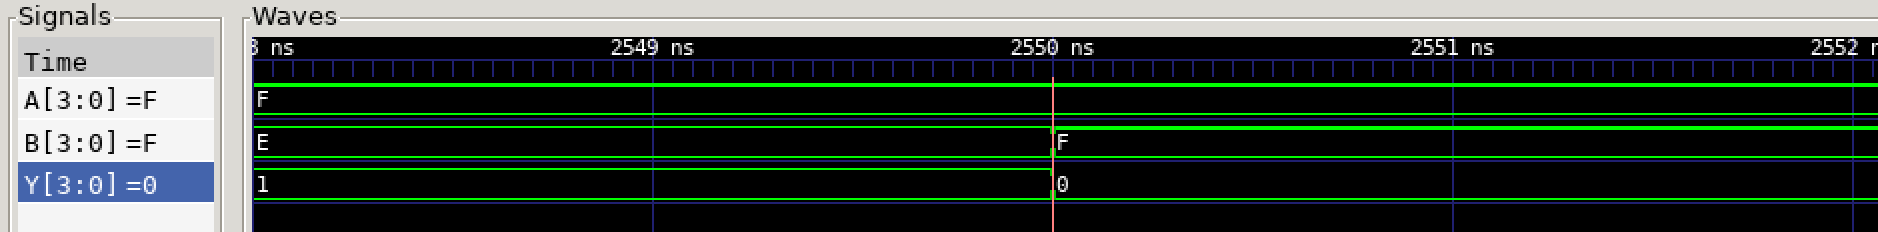
\includegraphics[width = 1.0\textwidth]{Xor/xor_wave2.png}
 \caption{Xor Circuit with marker at 2500ns}
 \label{fig:enter-label}
 \end{figure}

 \section{XNor Circuit}
 The Xnor circuit takes two 4-bit inputs A and B, with a 4-bit output Y. A and B will undergo the bitwise Xnor operation, and the result will be output to Y.
 \lstinputlisting[language=Verilog]{Xnor/xnor_gate.v} 
 
 To test the Xnor circuit, we have created two registers A and B, as well as a wire Y. We give the circuit some test cases to test its validity. We will know that our Xnor circuit is behaving as expected if Y produces correct values for all combinations of A and B. For example, if A = 1010 and B = 1101, the expected result for Y is 1000.
 \lstinputlisting[language=Verilog]{Xnor/xnor_tb.v}
 
 \subsection{Xnor Circuit Waveform} 
 
 At 1ns, A and B are both 0h (0000), so Y is Fh(0000).
 \begin{figure}[H]
  \centering
  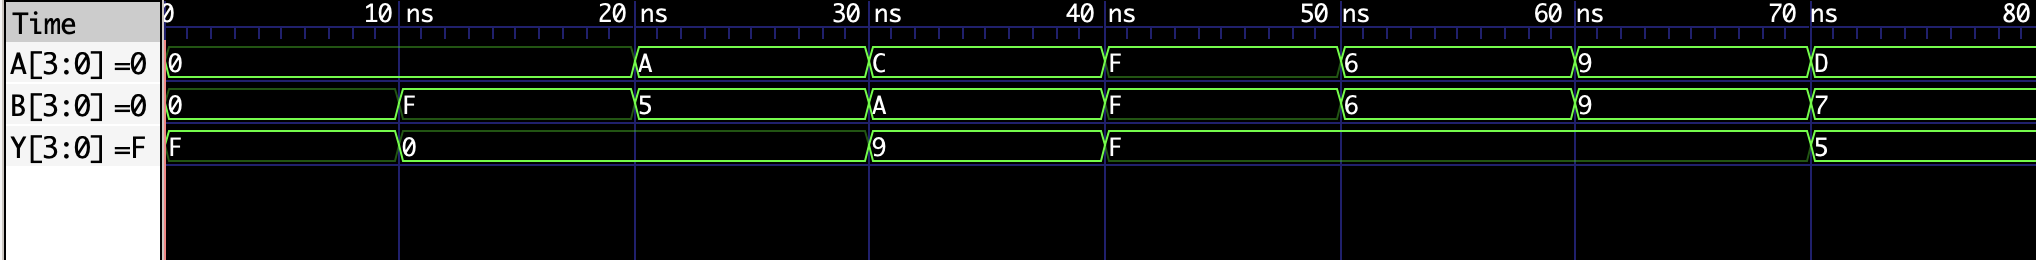
\includegraphics[width = 1.0\textwidth]{Xnor/XNOR-0ns.png}
  \caption{Xnor Circuit with marker at 1ns}
  \label{fig:enter-label} 
 \end{figure} 
 
 At 20ns, A = Ah (1010) and B = 5h(0101), so Y = 0h (0000).
  \begin{figure}[H]
  \centering 
 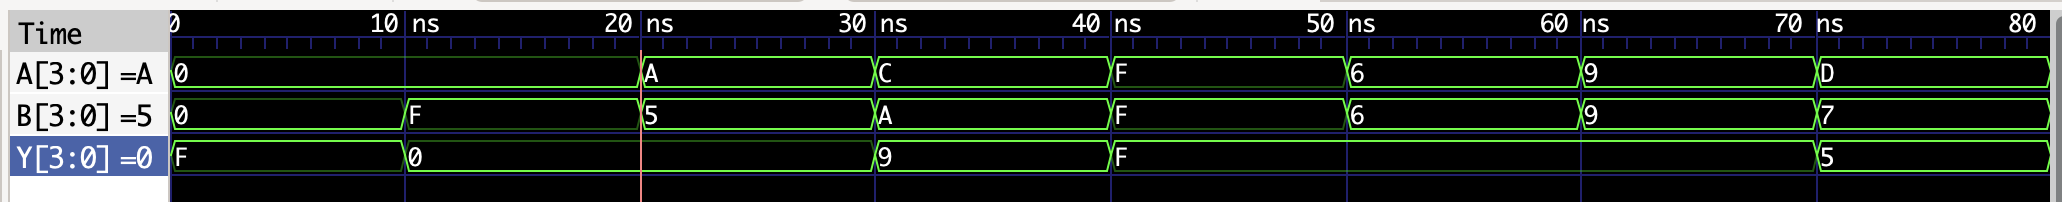
\includegraphics[width = 1.0\textwidth]{Xnor/XNOR-20ns.png}
  \caption{Xor Circuit with marker at 500ns}
  \label{fig:enter-label}
  \end{figure}
 
 At 40ns, A and B are both Fh(1111), so Y = Fh(1111).
  \begin{figure}[H]
  \centering 
 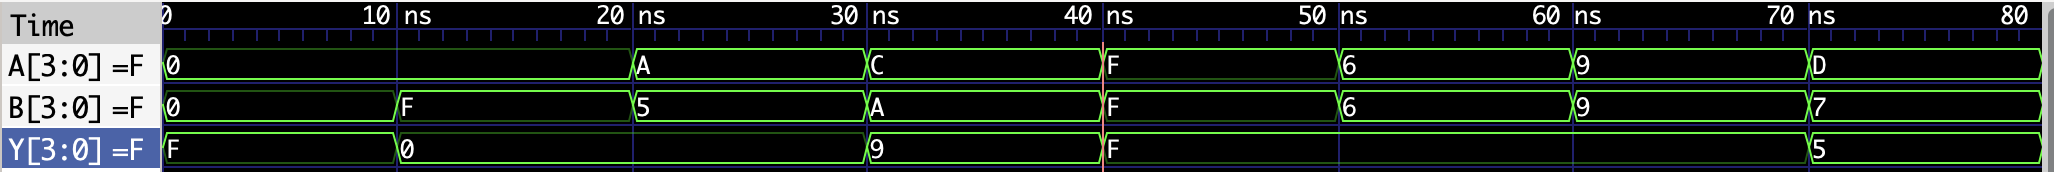
\includegraphics[width = 1.0\textwidth]{Xnor/XNOR-40ns.png}
  \caption{Xor Circuit with marker at 2500ns}
  \label{fig:enter-label}
  \end{figure}
 

\section{Addition Circuit}
The Addition circuit takes two 4-bit inputs A and B along with a 1-bit carry in to extend the output range from 15 to 31. The circuit’s outputs include  a 4-bit output called Sum, along with a 1-bit carry out to accommodate the extended range. The has an intermediary 5-bit variable, full sum, which is used to extract carry out and partial sum. First the full sum is found by adding A, B, and carry in. Then, Sum is assigned to the 4 lower bits of full sum. Then, carry out is assigned to the 5th bit of full sum. 
\lstinputlisting[language=Verilog]{Addition/addition.v}

To test the Addition circuit, we have created two registers A and B, a register carry in, a wire Sum, and a wire carry out. We then perform 5 tests with A, B, and carry in at various values. We will know that the Addition circuit is working as expected if carry out plus Sum produces correct results for every combination of A, B, and carry in that we have tested. For example, if A is 1000, B is 1000, and carry in is 1 , then the expected result: Sum is 0001, carry out is 1 for a decimal value of 17.
\lstinputlisting[language=Verilog]{Addition/addition_tb.v}
\subsection{Addition Circuit Waveform} 

At 2ns, A is 1 and B is 2, so Sum is 3 with  carry in and carry out at 0.

\begin{figure}[H]
 \centering
 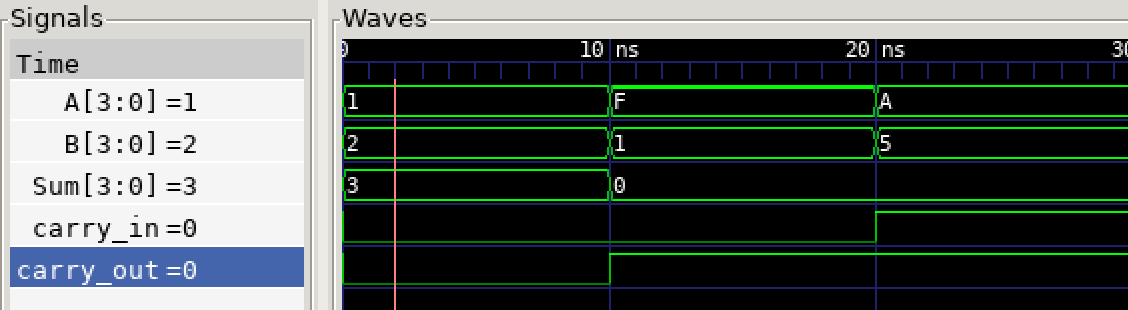
\includegraphics[width = 1.0\textwidth]{Addition/addition_wave.png}
 \caption{Addition Circuit with marker at 2ns}
 \label{fig:enter-label} 
\end{figure} 

At 20ns, A is A(1010) and B is 5(0101), so Sum is F(1111) with carry in and carry out at 0.
 \begin{figure}[H]
 \centering 
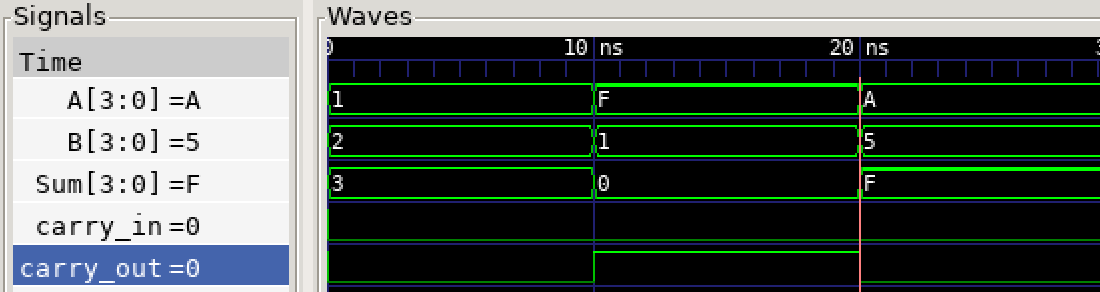
\includegraphics[width = 1.0\textwidth]{Addition/addition_wave1.png}
 \caption{Addition Circuit with marker at 20ns}
 \label{fig:enter-label}
 \end{figure}

 At 30ns, A and B are both 8(1000), so Sum is 1 with carry in and carry out at 1, resulting in a decimal value of 17.
 \begin{figure}[H]
 \centering 
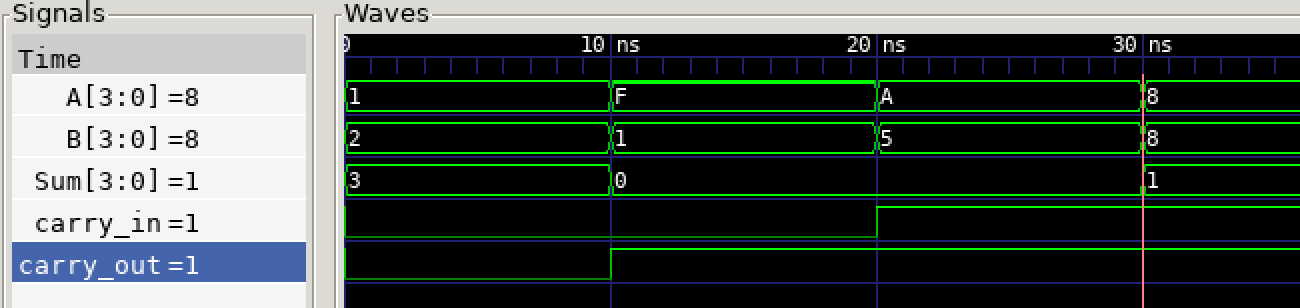
\includegraphics[width = 1.0\textwidth]{Addition/addition_wave2.png}
 \caption{Addition Circuit with marker at 30ns}
 \label{fig:enter-label}
 \end{figure}

\section{Multiplication Circuit}
The Multiplication circuit takes two 4-bit inputs A and B, and produces two 4-bit outputs, product low and product high, representing the high and low 4 bits of the product of A and B. The circuit has an intermediary 8-bit variable, full product, which is used to extract the low and high 4 bits of the product. First, full product is assigned to the product of A and B. Then, product low is assigned the first 4 bits of full product. Then, product high is assigned the last 4 bits of full product. 
\lstinputlisting[language=Verilog]{Multiplication/multiplication.v} 

To test the Multiplication circuit, we have created two registers A and B,and two wires product low and product high. We then perform 5 tests with A and B at various values. We will know that the Multiplication circuit is working as expected if product low, product high produces correct results for every combination of A times B that we have tested. For example, if A is 1111 and B is 1111, then the expected result: product high is 1110, product low is 0001 for a decimal value of 225.
\lstinputlisting[language=Verilog]{Multiplication/multiplication_tb.v}
\subsection{Multiplication Circuit Waveform} 

At 2ns, A is 2 and B is 3, so product high is 0 and product low is 6.  
\begin{figure}[H]
 \centering
 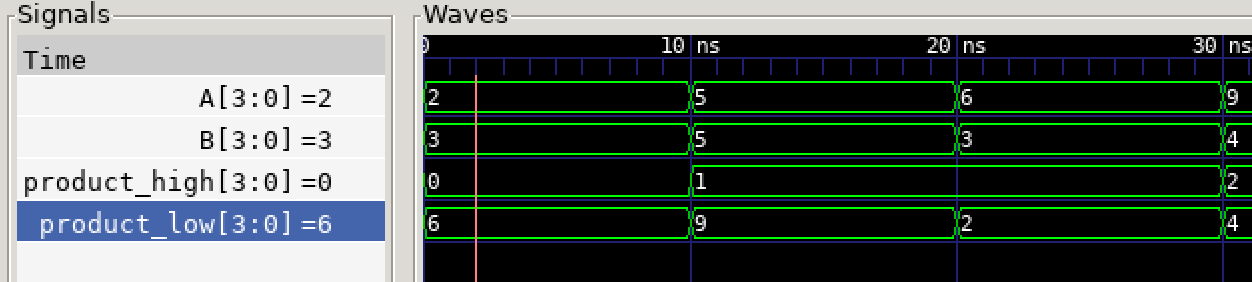
\includegraphics[width = 1.0\textwidth]{Multiplication/multiplication_wave.png}
 \caption{Multiplication Circuit with marker at 2ns}
 \label{fig:enter-label} 
\end{figure} 

At 20ns, A is 6 and B is 3, so product upper is 0001 and product lower is 0010 for a decimal value of 18.  
 \begin{figure}[H]
 \centering 
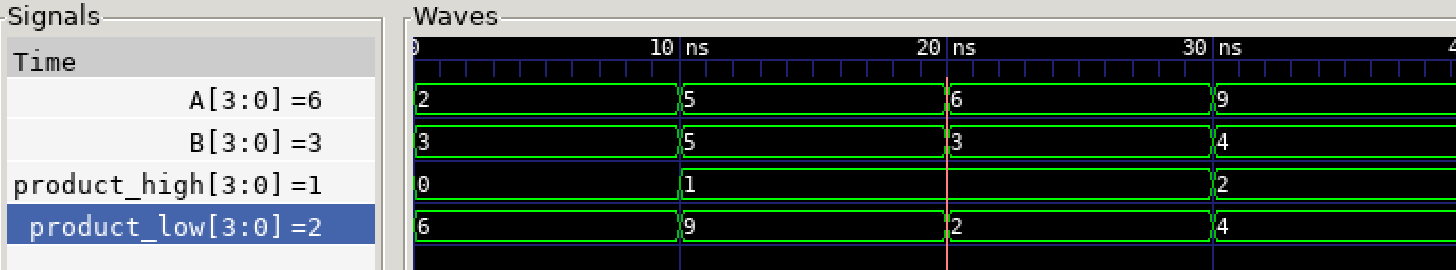
\includegraphics[width = 1.0\textwidth]{Multiplication/multiplication_wave1.png}
 \caption{Multiplication Circuit with marker at 20ns}
 \label{fig:enter-label}
 \end{figure}

 At 40ns, A and B are both F, so product upper is E and product lower is 0001 for a decimal value of 256.
 \begin{figure}[H]
 \centering 
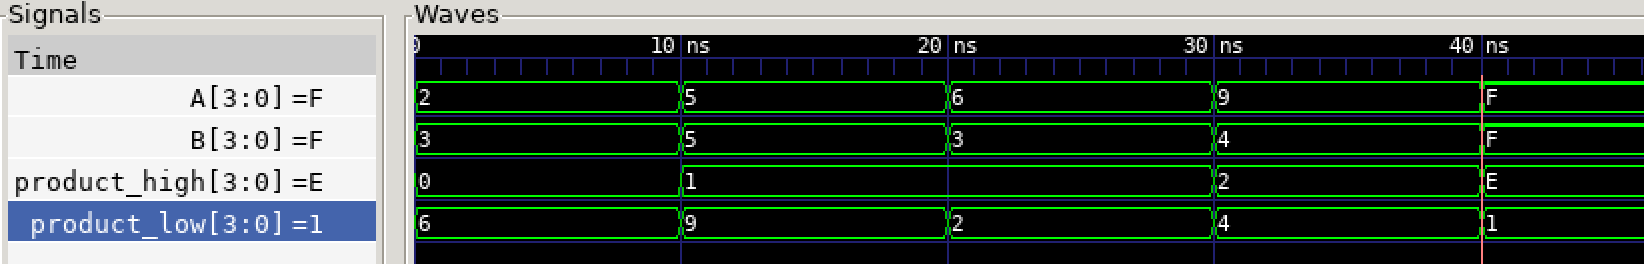
\includegraphics[width = 1.0\textwidth]{Multiplication/multiplication_wave2.png}
 \caption{Multiplication Circuit with marker at 40ns}
 \label{fig:enter-label}
 \end{figure}

\section{Subtraction Circuit}
\subsection{Subtraction Circuit Verilog Code} 
%The Multiplication circuit takes two 4-bit inputs A and B, and produces two 4-bit outputs, product low and product high, representing the high and low 4 bits of the product of A and B. The circuit has an intermediary 8-bit variable, full product, which is used to extract the low and high 4 bits of the product. First, full product is assigned to the product of A and B. Then, product low is assigned the first 4 bits of full product. Then, product high is assigned the last 4 bits of full product. 
\lstinputlisting[language=Verilog]{Subtraction/subtraction.v} 

%To test the Multiplication circuit, we have created two registers A and B,and two wires product low and product high. We then perform 5 tests with A and B at various values. We will know that the Multiplication circuit is working as expected if product low, product high produces correct results for every combination of A times B that we have tested. For example, if A is 1111 and B is 1111, then the expected result: product high is 1110, product low is 0001 for a decimal value of 225.
\lstinputlisting[language=Verilog]{Subtraction/subtraction_tb.v}
\subsection{Subtraction Circuit Waveform} 

At 0ns, A is 1h (0001) and B is 1h (0001), so Y = 0h (0000)  
\begin{figure}[H]
 \centering
 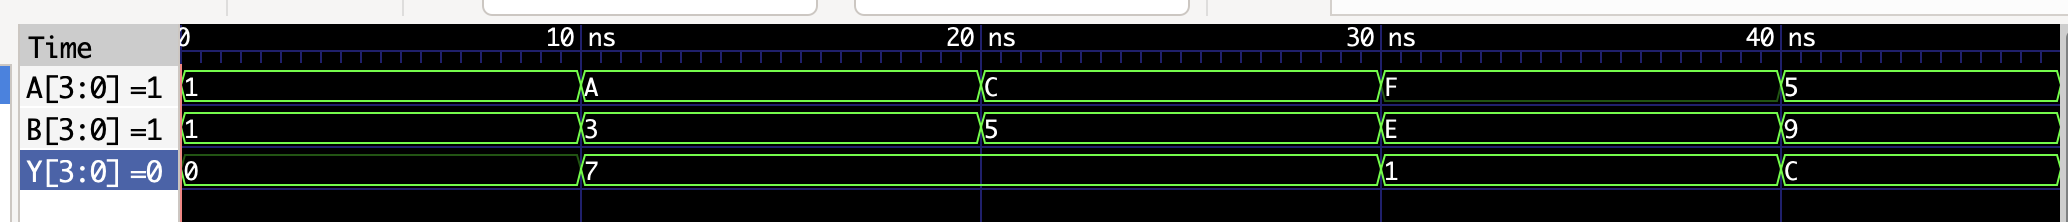
\includegraphics[width = 1.0\textwidth]{Subtraction/Subtraction-0ns.png}
 \caption{Subtraction Circuit with marker at 0ns}
 \label{fig:enter-label} 
\end{figure} 

At 0ns, A is Ch (1100) and B is 5h (0101), so Y = 7h (0111)  
 \begin{figure}[H]
 \centering 
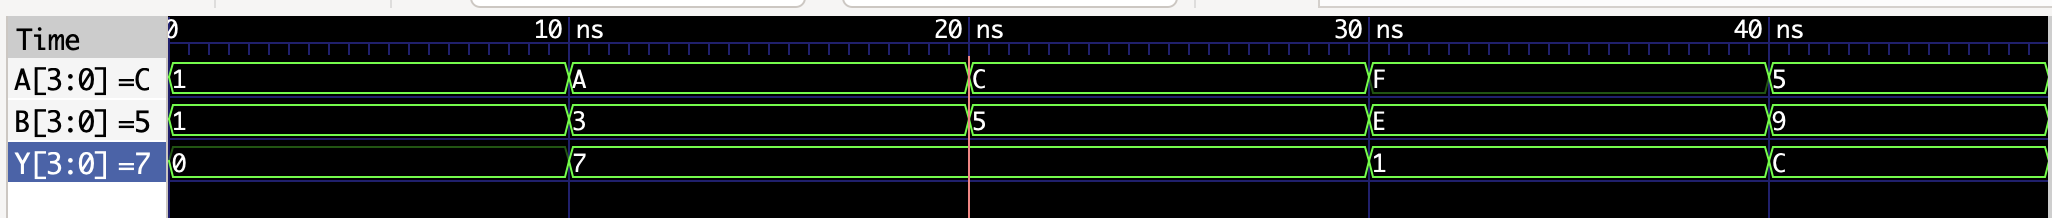
\includegraphics[width = 1.0\textwidth]{Subtraction/Subtraction-20ns.png}
 \caption{Subtraction Circuit with marker at 20ns}
 \label{fig:enter-label}
 \end{figure}

 At 0ns, A is 5h (0101) and B is 9h (1001), so Y = Ch (1100)  
 \begin{figure}[H]
 \centering 
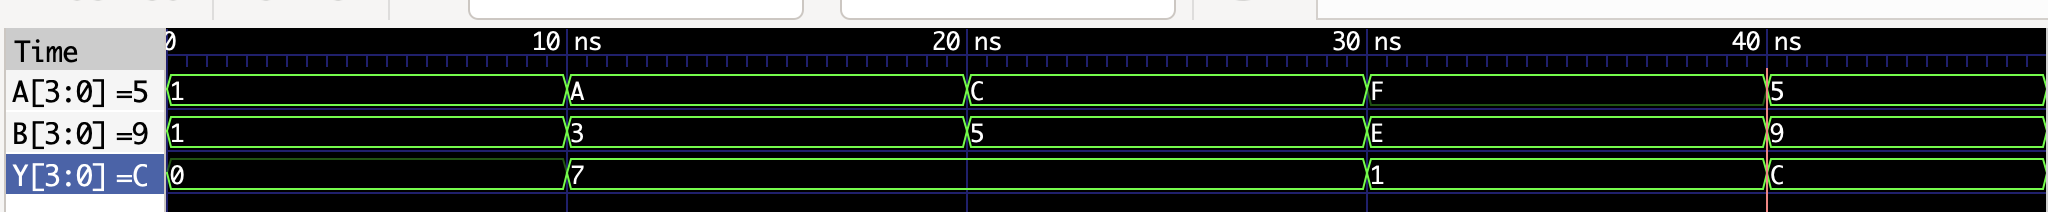
\includegraphics[width = 1.0\textwidth]{Subtraction/Subtraction-40ns.png}
 \caption{Multiplication Circuit with marker at 40ns}
 \label{fig:enter-label}
 \end{figure}


\section{Conclusion}

This project introduced the design and testing of a basic 4-bit Arithmetic Logic Unit (ALU). We coded essential logic functions like AND, OR, and NOT, along with shifting operations, which are crucial for handling binary data. We also developed basic arithmetic operations—addition, subtraction, multiplication, and division—which included handling carries and remainders to ensure accurate results.

Testing the circuits and generating waveforms confirmed that our ALU worked correctly across different inputs. This process highlighted the importance of both accuracy in coding and thorough testing. Overall, the project has been valuable for understanding digital circuits and the structure of an ALU, preparing us for more advanced digital logic design.
\end{document}



